\section{Results}
\label{sec:results}
We evaluate our method on several scenes consisting of procedurally generated mass models. 
%created with procedural extrusions~\cite{Kelly:SIGA:2017}.
We qualitatively show the fidelity of our output and the effects of style and scale control. Style and scale control are also evaluated quantitatively with a perceptual study, and we provide comparisons to existing end-to-end networks, both qualitatively and quantitatively through another perceptual study. 

\begin{figure*}[t!]
    \centering
    \includegraphics[width=\textwidth]{images/london.pdf}
    \caption{Detailed London area. The output of our method is shown on top, and the input style images at the bottom left. This is followed, from left to right, by close-ups of the input mass models, detail geometry generated by our method, and two detailed views of the generated model using super-resolution textures.}
    \label{fig:london}
\end{figure*}

\subsection{Datasets and Training Setup}

Each GAN in our framework performs an image-to-image transformation that is trained with a separate dataset of matched image pairs. Matched images for these pairs are obtained from three datasets:

The \emph{facade} dataset consists of the CMP dataset~\cite{cmp_dataset} and a larger dataset of labeled facades that has not yet been released, but that has been made available to us by the authors. The combined dataset contains $3941$ rectified facades with labels for several types of details, including doors, windows, window sills, and balconies.
%
We further refined this dataset by removing heavily occluded facades and by annotating the height of a typical floor in each facade to obtain the real-world scale that our GANs are conditioned on, as described in Section~\ref{sec:gan_architecture}.
%
From this dataset, we create matched pairs of images for each GAN in the facade chain.
%: (facade mask, window layout)-pairs, (window layout, facade texture)-pairs, and (facade texture, full facade label)-pairs.

The \emph{roof} dataset consists of $585$ high-quality roof images with labeled roof area, ridge/valley lines, pitched windows and chimneys. The images are part of an unreleased dataset. We contracted professional labellers to create high-quality labels.
%
From this dataset, we created matched pairs of images for the two GANs in the roof chain.
%: (coarse roof label, detailed roof label)-pairs and (detailed roof label, roof texture)-pairs.

The \emph{window} dataset contains $1376$ rectified window images with labeled window areas and glass panes. These images were obtained from Google Street View, and high-quality labels were created by professional labellers.
%
From this dataset, we created matched pairs of images for the two GANs in the window chain. Examples from all datasets are shown in Figure~\ref{fig:dataset}.

In addition to these three datasets, the super-resolution GANs were trained with two separate datasets. These datasets were created from a set of high-quality roof/wall texture patches that was downloaded from the internet, for example, brick patterns or roof shingles, and blurring them by random amounts. The networks are then trained to transform the blurred image to the original image. We found that it increased the performance of our networks to add in a second texture at a random location in the image. This accounts for changes in the texture over a facade or roof that occur in natural images.

\begin{table}
\centering
\small

\caption{GAN statistics:
%Summary of \textsc{FrankenGANs};
the size of the training data (n), resolution (in pixels squared), number of epochs trained, and if the network takes style as input.}
%\multicolumn{5}{c}{\textsc{London}} \\
%\hline
%block & roofs & facades & windows & time (s) \\
%\hline

\begin{tabular}{ccccc}
\hline
& n & resolution & epochs & style \\
\hline
roof labels & 555 & 512 & 400 & yes \\
roof textures & 555 & 512 & 400 & yes \\
facade window labels & 3441 & 256 & 400 & yes \\
facade textures & 3441 & 256 & 150 & yes \\
facade full labels & 3441 & 256 & 335 & no \\
window labels & 1176 & 256 & 200 & yes \\
window textures & 1176 & 256 & 400 & yes \\
facade super-resolution & 2015 & 256 & 600 & yes \\
roof super-resolution & 1122 & 256 & 600 & yes \\
\hline
\end{tabular}

\label{table:net_statistics}
\end{table}

To train each GAN, we alternate between discriminator optimization steps that minimize Eq.~\ref{eq:loss_gan_d} and generator/encoder optimization steps that minimize Eq.~\ref{eq:loss_gan}. The optimization is performed with Adam~\cite{adam}. The weights $(\lambda_{\textrm{GAN}}, \lambda_{\textrm{L1}}, \lambda_{\textrm{KL}}, \lambda_{\textrm{LR}})$ in Equation~\ref{eq:loss_gan} are set to $(1, 10, 0.01, 0.5)$. A large $\lambda_{\textrm{L1}}$ encourages results that are close to the average over all training images. This helps to stabilize training for textures. For label map generation, however, there is usually one dominant label, such as the wall or the roof label, and a large $L1$ loss encourages the generation of this label over other labels. Lowering the $L1$ loss to $1$ improves results for label maps.
% also update GAN architecture section to include the final sum of energy terms with weights
% and maybe discuss the tradeoff between l1 weight and discriminator there? (that L1 should be small for label map generation), but probably better only here
% unbias L1 weight for:
% - image2celabels
% lower L1 weight for:
% - w3_empty2labels
% - r3_clabels2labels
% - empty2windows
Statistics for our GANs are summarized in Table~\ref{table:net_statistics}.

At test time, we evaluate our networks on mass models created through procedural reconstruction from photogrammetric\linebreak meshes~\cite{Kelly:SIGA:2017}. Facades and roofs on these mass models are labeled, and roof ridges and valleys are known, providing all necessary inputs for \systemName: facade masks and coarse roof label maps. Note that it obtaining these inputs automatically from any type of reasonably clean mass model, is also feasible.

\begin{figure*}[t!]
    \centering
    \includegraphics[width=\textwidth]{images/madrid.pdf}
    \caption{Detailed Madrid area. Input style images and mass models are shown on the left, an overview of our output in the center, and close-ups of our output and the generated geometry (green), showing details like balconies and window moldings, on the right. Lower right panel uses  super-resolution textures.}
    \label{fig:madrid}
\end{figure*}


\subsection{Qualitative Results}


We show the quality of our results with one area of Madrid and one area of London, both spanning several blocks. As our reference style, we take images of facades, windows and roofs, some of which are taken from our dataset, and some from the web. Figures~\ref{fig:teaser} and \ref{fig:london} show the result of detailing the London scene. Reference style textures and input mass models are shown on the left, our detailed result on the right. We produce varied details that are not completely random, but guided by the style given as input. In this example, several sets of style textures are used. Note the varied window layouts and textures: each building has unique layouts and textures that are never repeated. 

Figure~\ref{fig:madrid} shows our results of detailing the Madrid scene. Reference style images and a detailed view of the input mass models are shown on the left; our output is shown in the center and on the right, including a detailed view of the generated geometry. Note several modes of matching styles in the result, including red buildings with black roofs and yellow buildings that often have several ledges.

\begin{table}
\centering

\setlength{\tabcolsep}{1.5pt}

\caption{Statistics for the London and Madrid scenes. We show the number of roofs, facades and windows in each block, as well as the time taken to generate the block.}
\footnotesize
\begin{minipage}{.49\columnwidth}
\begin{tabular}{cccccc}
\multicolumn{5}{c}{\textsc{London}} \\
\hline
block & roofs & facades & windows & time(s) \\
\hline
1 & 29 & 145 & 1075 & 490 \\
2 & 20 & 204 & 541 & 351 \\
3 & 15 & 87 & 536 & 222 \\
4 & 25 & 133 & 1040 & 400 \\
5 & 47 & 243 & 2107 & 809 \\
6 & 27 & 171 & 1622 & 597 \\
7 & 10 & 65 & 1144 & 403 \\
8 & 7 & 40 & 559 & 199 \\
9 & 8 & 42 & 786 & 271 \\
10 & 26 & 158 & 1566 & 577 \\
\hline
\textbf{total} & 214 & 1288 & 10976 & 4322 \\
\hline
\end{tabular} 
\end{minipage}
%
\hfill
%\hspace{1pt}
%
\begin{minipage}{.49\columnwidth}
\begin{tabular}{cccccc}
%\multicolumn{5}{c}{ } \\
\multicolumn{5}{c}{\textsc{Madrid}} \\
\hline
block & roofs & facades & windows & time(s) \\
\hline
1 & 22 & 146 & 773 & 315 \\
2 & 20 & 110 & 559 & 239 \\
3 & 17 & 103 & 471 & 219 \\
4 & 12 & 67 & 399 & 166 \\
5 & 7 & 66 & 230 & 102 \\
6 & 22 & 116 & 758 & 291 \\
7 & 25 & 139 & 571 & 292 \\
8 & 22 & 125 & 611 & 255 \\
9 & 35 & 240 & 1219 & 495 \\
10 & 37 & 222 & 738 & 350 \\
\hline
\textbf{total} & 219 & 1334 & 6329 & 2722 \\
\hline
\end{tabular}
\end{minipage}

\vspace{-5pt}

\label{table:scene_statistics}
\end{table}

Statistics for the London and Madrid scenes are shown in Table~\ref{table:scene_statistics}. Each of the scenes has $10$ blocks and contains an average of $21$ buildings (the number of buildings equals the number of roofs). All of the generated details, including their textures, are unique in the entire scene. In the London scene, we generate approximately $860$ Megapixels of texture and $2.68$ million triangles; in the Madrid scene we generate approximately $560$ Megapixels and $1.17$ million triangles. The time taken to generate the scenes on a standard desktop PC with an Intel 7700k processor, 32 GB of main memory, and an NVidia GTX 1070 GPU is shown in the last column of Table~\ref{table:scene_statistics}. The \systemName implementation has two modes - when minimizing GPU memory, a single network is loaded at a time, and all applicable tasks in a scene are batch processed; when GPU memory is not a constraint, the whole network can be loaded at once. These modes use 560 MB and 2371 MB of GPU memory, respectively, leaving sufficient space on the graphics card to interactively display the textures. These figures compare favourably with larger end-to-end networks that require more memory~\cite{Karras:2018:PGG}.

%Figure \ref{fig:teaser} has 1.78 million verts, 2.68m triangles. 
%It has 7306 bitmaps 256x256 maps - rgb, normals and specular. The system used for these timings (and used in the video) was a standard video-gaming desktop (Intel 7700k, 32Gb, and an NVidia 1070). The graphics card drove both the interactive previews and the GANs.

\subsection{Qualitative Comparisons}
\label{sec:qualitative_comparisons}
In this section, we qualitatively evaluate the style control of \systemName and compare our results to two end-to-end GANs: Pix2Pix~\cite{pix2pix} and BicycleGAN~\cite{zhu2017multimodal}. Similar quantiative evaluations and comparisons, based on two perceptual studies, are provided in the next section.

\begin{figure*}[t]
    \centering
    \includegraphics[width=\textwidth]{images/eval_style_control.pdf}
    \caption{Different types of style distributions. From left to right, a constant style is used for all houses, a style chosen randomly from the style prior, a style sampled independently for all building properties, and a dependently sampled property style. Note that in the last two columns, there are several separate modes for properties, such as wall and building color, that are either mixed randomly for each building (third column) or sampled dependently (last column).}
    \label{fig:eval_style_control}
\end{figure*}

\begin{figure}[b]
    \centering
    \includegraphics[width=\columnwidth]{images/super_style.pdf}
    \caption{Different super-resolution styles. The original low-resolution facade and roof textures are shown on the left; the middle and right buildings show two different super-resolutions styles, resulting in different textures for the roof tiles or stone wall.}
    \label{fig:super_style}
\end{figure}

To evaluate the effects of style control on our outputs, we compare four different types of style distributions applied to similar mass models in Figure~\ref{fig:eval_style_control}. On the left, a constant style vector is used for all houses. This results in buildings with similar style, which may, for example, be required for row houses or blocks of apartment buildings. A fully random style is obtained by sampling the style prior, a standard normal distribution. The diversity in this case approximates the diversity in our training set. Using a Gaussian mixture model (GMM) as the style distribution, as described in Section~\ref{sec:style_control}, gives more control over the style. Note the two modes of white and red buildings in the third column, corresponding to two reference style images. The style for different building properties, such as roof and facade textures, is sampled independently, resulting in randomly re-mixed property styles, both white and red facades, for example, are mixed with black and red roofs. When specifying multiple sets of GMMs, one set is randomly picked for each house, allowing the user to model dependencies between property styles, as shown in the last column.

Examples of different super-resolution styles are shown in Figure~\ref{fig:super_style}. Since a low-resolution texture contains little information about fine texture detail, like the shingles on a roof or the stone texture on a wall, there is a diverse range of possible styles for this fine texture detail, as shown in the middle and right building.

\begin{figure*}[t]
    \centering
    \includegraphics[width=\textwidth]{images/qual_comparison.pdf}
    \caption{Qualitative comparison with end-to-end GANs. The left column shows results of Pix2Pix trained to transform empty facade and roof masks to textures. The middle column shows BicycleGAN trained similarly, while the last column shows our method. Note how Pix2Pix suffers from mode collapse, while BicyleGAN has less realistic window layouts and lacks scale and style consistency. \systemName provides better style control and our approach of splitting up the problem into multiple steps opens up several avenues to increase the realism of our models.}
    \label{fig:qual_comparison}
\end{figure*}

Figure~\ref{fig:qual_comparison} shows a qualitative comparison to Pix2Pix and BicycleGAN. We trained both end-to-end GANs on our facade and roof datasets, transforming empty facade and roof masks to textures in one step. As discussed in Section~\ref{sec:gan_architecture}, Pix2Pix, like most image-to-image GANs, has low output diversity for a given input image. In our case, the input image, being a blank facade or roof rectangle, does not provide much variation either, resulting in a strong mode collapse for Pix2Pix, shown by the repeated patterns such as the `glass front' pattern across multiple buildings. Like \systemName, BicycleGAN takes a style vector as input, which we set to a similar multi-modal distribution as in our method. There is more diversity than for Pix2Pix, but we observe inconsistent scale and style across different buildings, or across different facades of the same building, less realistic window layouts, and less diversity than in our results. Splitting the texture generation task into multiple steps allows us to provide more training signals, such as an explicit ground truth for the window layout, without requiring a very large network, regularize the intermediate results of the network and then use the intermediate results as label maps that can be used to generate geometric detail and assign materials. Additionally, giving the user more precise control over the style results in more consistent details across a building or parts of buildings. This allows us to generate more diverse and realistic building details. In the next section, we quantify the comparison discussed here with a perceptual study.


\subsection{\changed{Perceptual} Studies}

\begin{figure}[b]
    \centering
    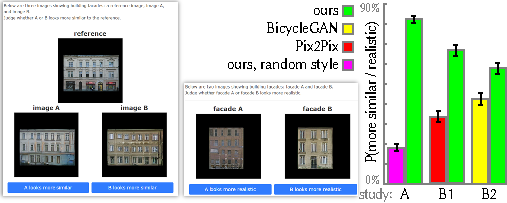
\includegraphics[width=\columnwidth]{images/study.pdf}
    \caption{Perceptual studies comparing our method with/without style guidance (left) and to Pix2Pix~\cite{pix2pix} and BicycleGAN~\cite{zhu2017multimodal} (middle). The average probability for each method of being judged more similar to the reference or more realistic by the study participants is shown on the right. The black bars are $95\%$ confidence intervals.}
    \label{fig:study}
\end{figure}

We performed two perceptual studies to quantify the following questions:
\begin{enumerate}[label=(\Alph*)]
\item \emph{How visible are the effects of style and scale control?}
\item \emph{How does the realism of \systemName compare with that of Pix2Pix~\cite{pix2pix} and BicycleGAN~\cite{zhu2017multimodal}?}
\end{enumerate}
To investigate question A, we tested if participants could reliably tell which of two generated facades was guided by a given reference style facade. The style and scale was randomized for the other facade.
%
Question B was investigated by comparing facades generated by \systemName and one of the other two methods side-by-side and asking participants to compare the realism of the two facades.
%
We performed both studies in Amazon Mechanical Turk (AMT). Screenshots of both studies are shown in Figure~\ref{fig:study}; \changed{the assignment of images to the left and right positions was randomized.}

For study A, we created $172$ triples of facades, each consisting of a reference facade, a facade with style and scale given by the reference facade, and a third facade with randomized style. Participants were asked which of the two facades was more similar to the reference. Each triple was evaluated by an average of $11$ participants, and a total of $116$ unique participants took part in the study. Figure~\ref{fig:study} (green vs. blue) shows the average probability of a participant choosing either the style-guided facade or the facade with randomized style as more similar to the reference facade. Our results show that style-guided facade was consistently chosen, implying good visibility of style and scale control.

The second study was performed in two parts. In the first part, we compare our method to Pix2Pix, and in the second part to BicycleGAN. Users were shown one facade generated with \systemName and one facade with the other method, trained end-to-end to transform facade masks to facade textures. Each pair was evaluated by an average of $17.6$ and $17.5$ users, for Pix2Pix and BicycleGAN, respectively, and there were $86$ unique participants in the study. Results are shown in Figure~\ref{fig:study} (red vs. blue and yellow vs. blue). \systemName was chosen as more realistic in $66.6\%$ of the comparisons with Pix2Pix and $57.6\%$ of the comparisons for BicycleGAN. $95\%$ confidence intervals are shown as small bars in Figure~\ref{fig:study}. Note that this advantage in realism is in addition to the advantage of of having fine-grained style and scale control and obtaining label maps as intermediate results that are necessary to generate 3D details.

\subsection{Limitations}

There are also some limitations to our framework. To replicate the framework from scratch requires extensive training data.
%while the GANs themselves is inherently difficult and requires experience.
%Exploring the training-parameter space of each dataset can involve several training runs.
Similar to other GANs, our results look very good from a certain range of distances, but there is a limit to how close it is possible to zoom in before noticing a lack of details \changed{or  blurriness}. This would require the synthesis of displacement maps and additional material layers in addition to textures. Data-driven texturing is inherently dependent on representative datasets. For example, our facade label dataset had missing windows due to occlusions by trees and other flora. We thus occasionally see missing windows in our results. We chose not to fill in windows in the regularisation stage.
%try to find these windows in the regularisation stage.
The facade-texturing network then learned to associate these missing windows with flora, and dutifully added green "ivy" to the building walls (Figure~\ref{fig:limitations}, left). Finally, our system uses a shared style to synchronize the appearance of adjacent building facades. However, this compact representation does not contain sufficient detail to guarantee seamless textures at boundaries (Figure~\ref{fig:limitations}, right).

\begin{figure}[b]
    \centering
    \includegraphics[width=\columnwidth]{images/limitations.pdf}
    \caption{Limitations. Green: the system is prone to generating green vegetation over missing windows. Red: texture discontinuities at boundaries.}
    \label{fig:limitations}
\end{figure}